%--- Implementation
\begin{figure}[h!]
    \centering
    \caption{Effects of \emph{Plan Cuadrante} on Reported Crime and Arrests (Sample of Municipalities Included in the Analysis of ENUSC Outcomes)}
    \label{fig:figure02_N47}
    \begin{subfigure}{0.495\textwidth}
        \centering
        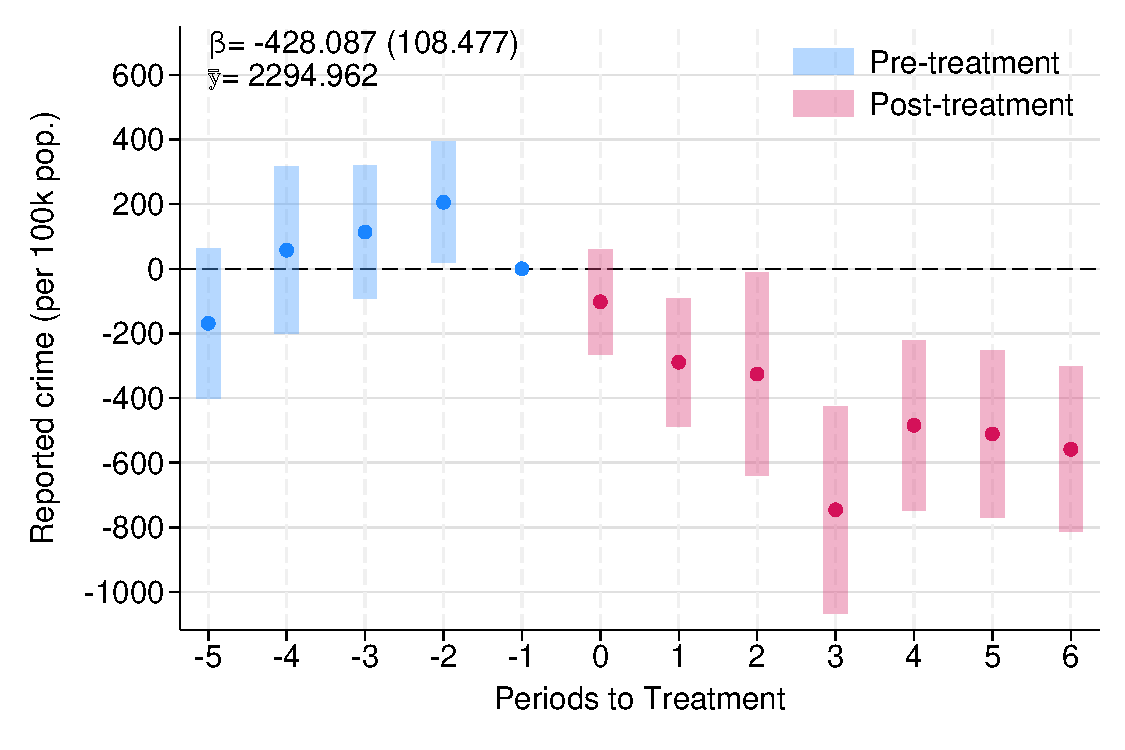
\includegraphics[width=\textwidth]{../manuscript/Graphs/totalreportedcrime_47enusc.pdf}
        \caption{Reported crime per 100k inhabitants}
    \end{subfigure}%
    ~ 
    \begin{subfigure}{0.495\textwidth}
    \centering
    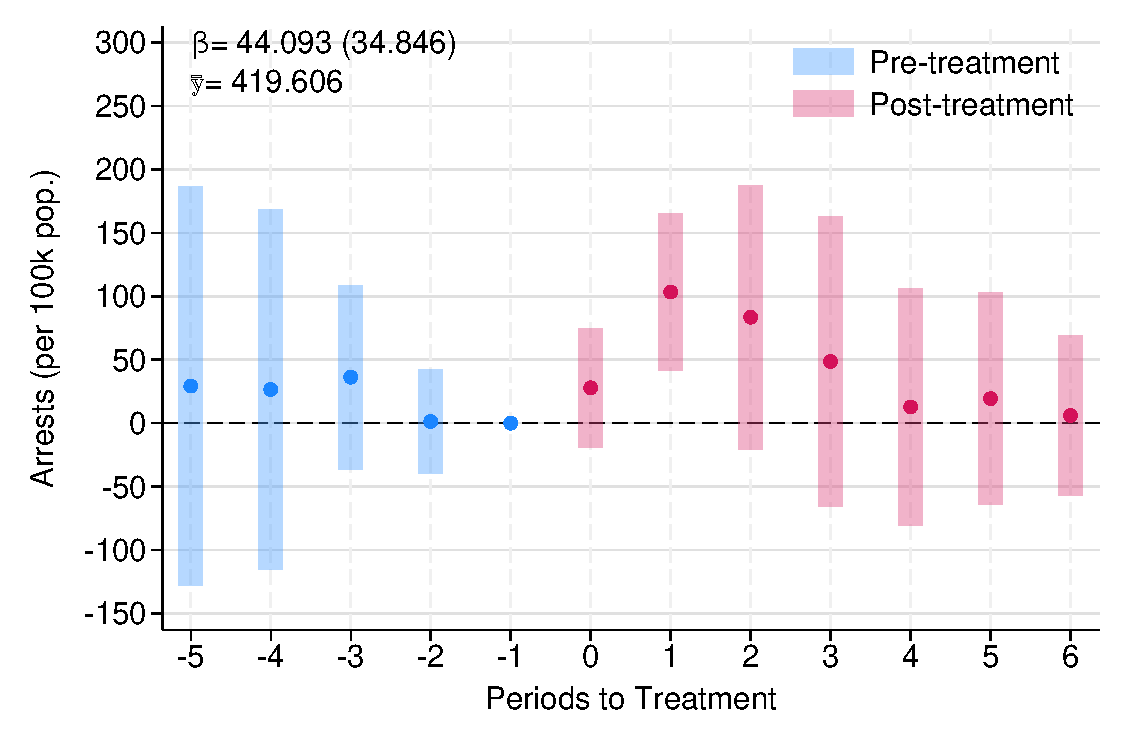
\includegraphics[width=\textwidth]{../manuscript/Graphs/totalarrestscrime_47enusc.pdf}
        \caption{Arrests per 100k inhabitants}
    \end{subfigure}
    \\[12pt]
    \begin{minipage}{0.99\textwidth}
    \footnotesize Notes: This figure shows the dynamic effects of \emph{Plan Cuadrante} on the number of crimes reported to the police per 100,000 inhabitants in the municipality in panel (a) and on the number of arrests per 100,000 inhabitants in the municipality in panel (b) using administrative data from the Undersecretary for Crime Prevention. The analysis is conducted using only the sample of municipalities included in the analysis of ENUSC outcomes. Panel (a) includes 592 observations, while panel (b) includes 405 observations. The estimation is conducted using the procedure developed in \citet{Callaway} for difference-in-differences with staggered treatment adoption. The dots in the figure represent the estimated coefficients and the bars behind them 95\% confidence intervals. Standard errors are clustered at the municipality level using wild bootstrapping. The pooled effect and the mean outcome before the introduction of the treatment is also presented in each panel. 
    \end{minipage}
\end{figure}
